\documentclass[10pt,a4paper]{article}
\usepackage[utf8]{inputenc}
\usepackage[T1]{fontenc}
\usepackage{amsmath}
\usepackage{amssymb}
\usepackage{graphicx}
\usepackage{hyperref}
\usepackage{float}
\usepackage{subcaption}
\usepackage{geometry}
\geometry{a4paper, margin=1in}

\title{Investigating the Platonic Representation Hypothesis}
\author{Aryasomayajula Ram Bharadwaj\\
Independent Researcher\\
\texttt{ram.bharadwaj.arya@gmail.com}}
\date{20th Oct 2024}

\begin{document}

\maketitle

\begin{abstract}
The Platonic Representation Hypothesis (PRH) \cite{huh2024prh} suggests that neural networks, despite being trained on different objectives, modalities, and datasets, tend to converge toward a shared statistical model of reality. This work investigates the specific conditions required for this phenomenon. Our results indicate that PRH holds even in out-of-distribution (OOD) contexts but faces limitations with random data, offering a nuanced view on representational alignment. Additionally, we examine how training duration and the signal present in data influence convergence toward this shared model.
\end{abstract}

\section{Introduction}
Understanding how neural networks form internal representations of the world is a key research area, bridging philosophy and machine learning. The Platonic Representation Hypothesis (PRH) \cite{huh2024prh}, inspired by Plato’s Allegory of the Cave, proposes that models across domains—such as vision or language—are converging toward a shared, idealized model of reality. According to PRH, even when trained on different datasets, models internalize similar structures, reflecting Plato’s concept of perceiving shadows of an underlying truth.

However, some key questions remain: does this convergence persist when models encounter data significantly different from their training distributions? How does data quality (in terms of signal and information) affect convergence to a shared statistical model? And how does convergence change with varying training progress? This study explores these questions by evaluating PRH under scenarios involving out-of-distribution (OOD) data, purely random data, and progressive noise levels, as well as during different stages of language model training.

\section{Methodology}
To evaluate PRH rigorously, we designed experiments that test the hypothesis under varied data distribution conditions. Our methodology centers on three main experimental setups, each focused on a distinct aspect of model alignment.

\subsection{Experimental Setup}
\textbf{1. Representational Alignment Across Data Types:} We measured alignment between different models across three scenarios: in-distribution, out-of-distribution, and purely random data using the following datasets:
\begin{enumerate}
    \item \textbf{In-distribution data}: The validation set from Places365, which closely aligns with the training data of many vision models. Results for this were adapted directly from the original study \cite{huh2024prh}.
    \item \textbf{Out-of-distribution data}: The ImageNet-O dataset, containing images that fall outside the standard ImageNet distribution \cite{hendrycks2021nae}. This allows examination of PRH in data with significant divergence.
    \item \textbf{Random noise}: A dataset of purely random images probes the extreme boundaries of representational alignment. Random noise vectors with matching dimensions to the original dataset were generated, helping assess whether models converge on a shared interpretation in the absence of structured input.
\end{enumerate}

Alignment was measured using Spearman's rank correlation on mutual k-NN distances across model representations, comparing how models interpret the similarity of various data inputs.

\subsection{Noise Injection in Vision Models}
\textbf{2. Progressive Noise Injection:} To understand the importance of signal quality or information content for representational alignment, we conducted a noise injection experiment:
\begin{itemize}
    \item A set of 250 images was progressively corrupted with Gaussian noise over 100 steps.
    \item At each noise level, we measured mutual alignment across 17 Vision Transformer models, evaluating changes in representational structures as noise increased.
    \item Alignment scores were analyzed to detect non-linear relationships and patterns in how noise impacts convergence.
\end{itemize}

\subsection{Tracking Alignment During Language Model Training}
\textbf{3. Evolution of Alignment During Training:} We also studied how representational alignment evolves during language model training:
\begin{itemize}
    \item Six large language models (LLMs) were analyzed using checkpoints saved at 100 different training stages.
    \item At each checkpoint, alignment was measured between every pair of models to observe changes in representational similarity over time.
    \item This analysis aimed to uncover phases of increased or decreased similarity, providing insights into how models internalize structure across training stages.
\end{itemize}

\section{Results}
\subsection{Alignment Across Data Types}
\begin{figure}[H]
    \centering
    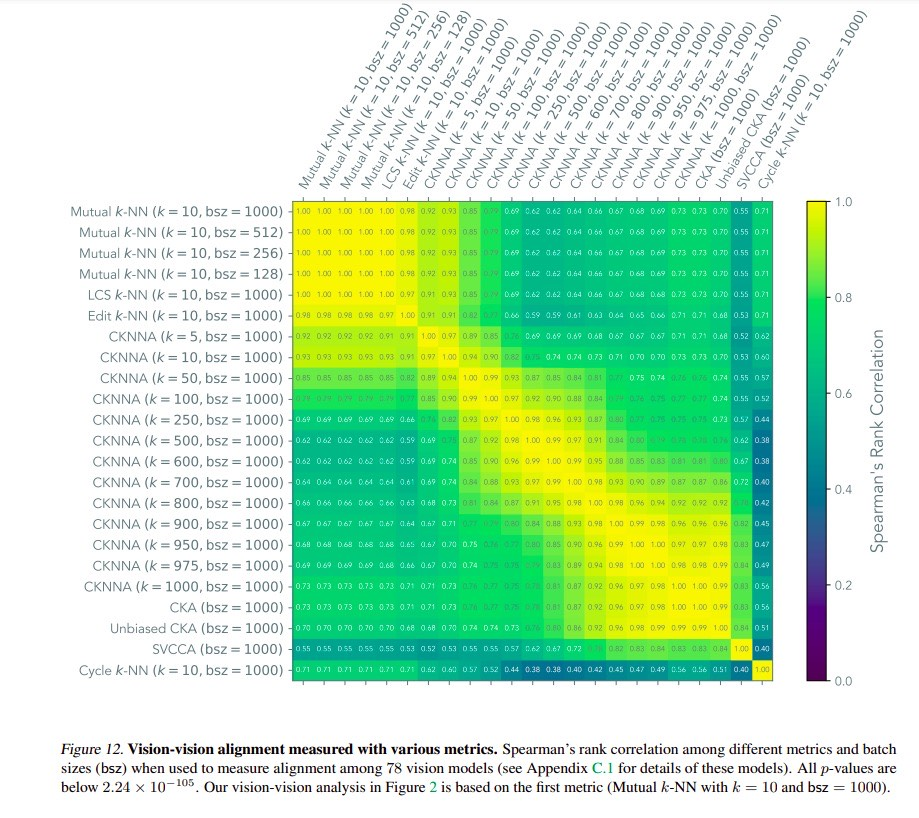
\includegraphics[width=\textwidth]{prh_correlation.jpg}
    \caption{Spearman rank correlation between models on Places365's validation data, indicating a high degree of alignment in in-distribution data.}
    \label{fig:prh_correlation}
\end{figure}

\subsection{Alignment on ImageNet-O Data}
\begin{figure}[H]
    \centering
    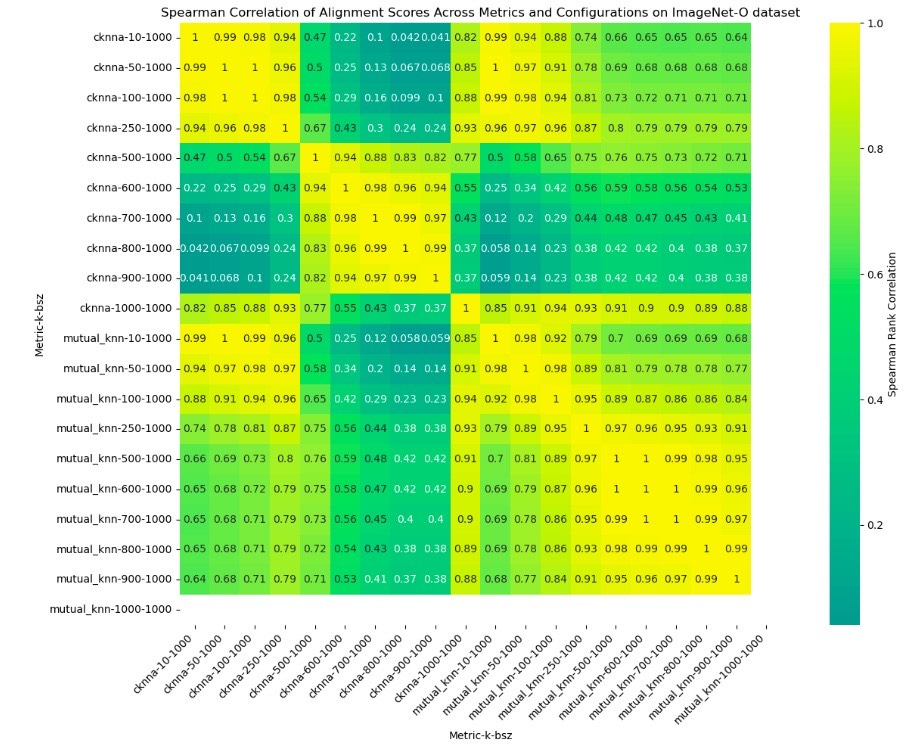
\includegraphics[width=\textwidth]{prh_correlation_ood.jpg}
    \caption{Alignment of vision models on the ImageNet-O dataset. Spearman correlation suggests that even with outlier data, models maintain shared statistical representation. Despite prediction errors in this OOD case, models converge in their representations, implying that larger models exhibit predictable error patterns similar to smaller models.}
    \label{fig:prh_correlation_ood}
\end{figure}

\subsection{Alignment on Random Noise Data}
\begin{figure}[H]
    \centering
    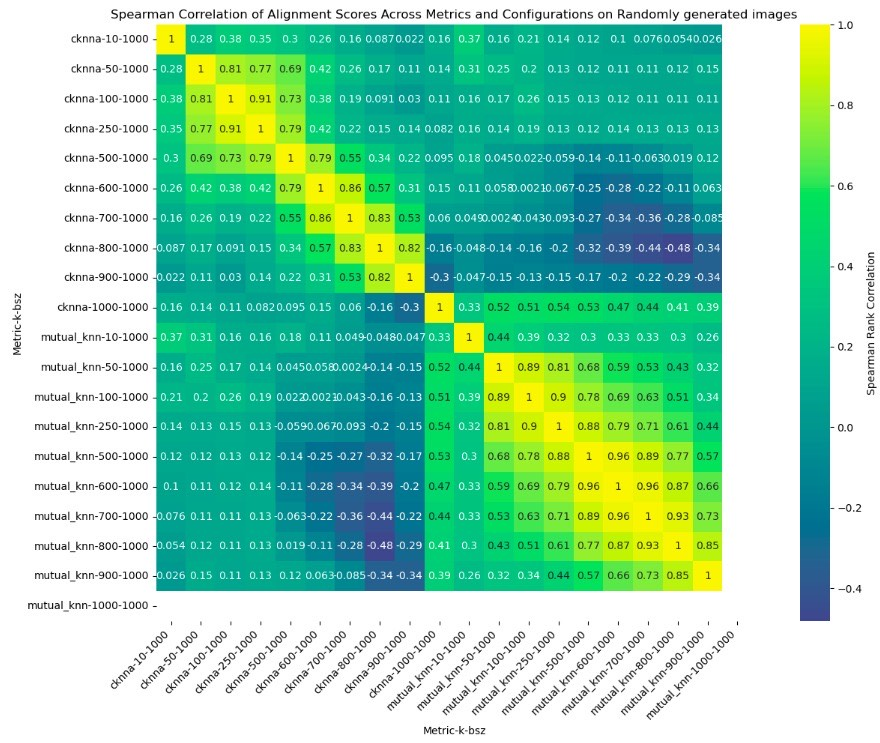
\includegraphics[width=\textwidth]{prh_correlation_random.jpg}
    \caption{Spearman correlation of alignment scores on random noise data. The lower correlation values indicate a breakdown in representational alignment, suggesting that random data lacks the underlying structure required for PRH. This suggests that representational alignment, while present in OOD cases, still depends on some structural properties within the dataset.}
    \label{fig:prh_correlation_random}
\end{figure}

\subsection{Impact of Noise Injection}
\begin{figure}[H]
    \centering
    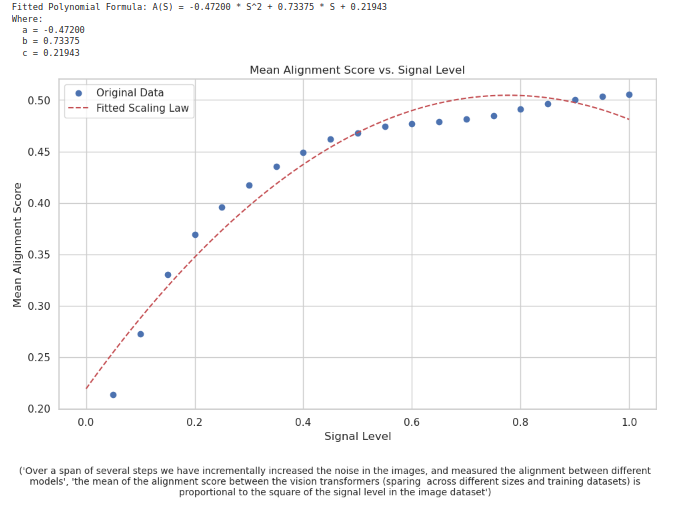
\includegraphics[width=\textwidth]{alignment_vs_signal_level.png}
    \caption{Relationship between noise level and mean alignment scores of 17 ViT models. A quadratic trend is observed as noise increases. Noise was progressively added to the dataset, with alignment scores calculated at each stage. The results suggest a threshold of signal required for representational alignment to occur. Alignment follows a smooth trend proportional to the square of the signal quantity present in the model.}
    \label{fig:alignment_vs_signal_level}
\end{figure}

\clearpage

\begin{figure}[H]
    \centering
    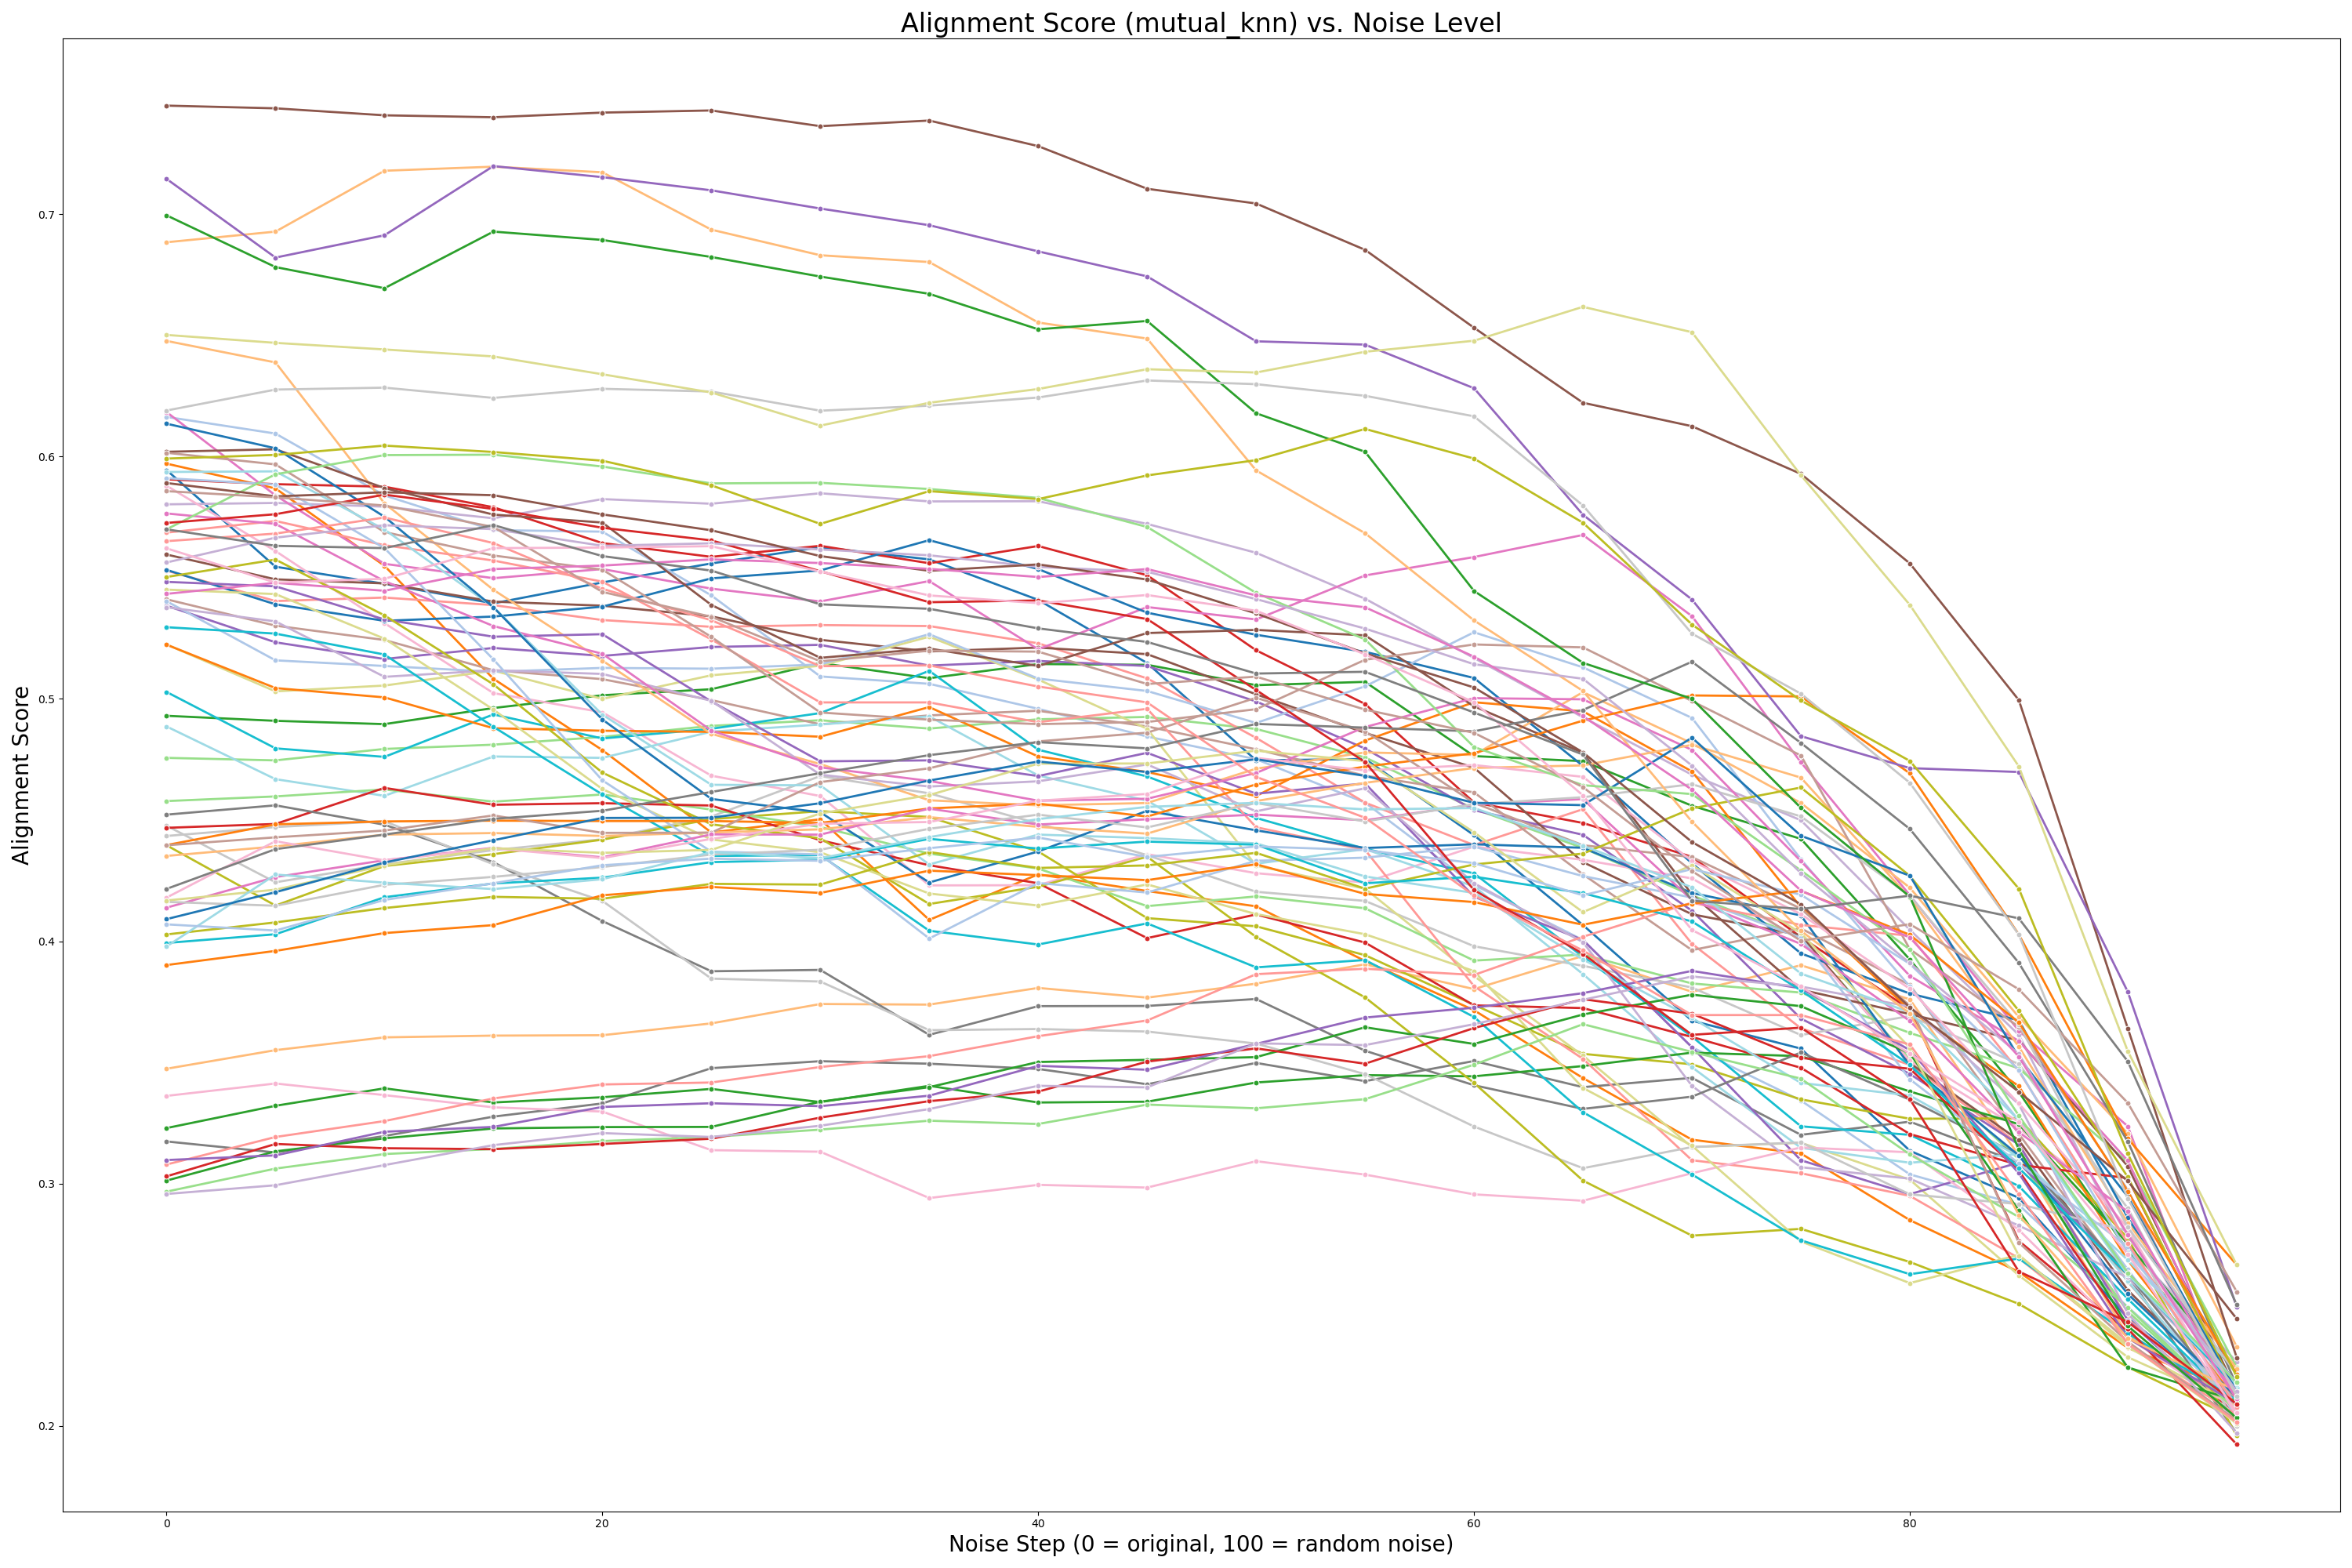
\includegraphics[width=\textwidth]{alignment_plot.png}
    \caption{Alignment of individual ViT models with respect to noise level. This plot provides a detailed view of how each model’s representational alignment responds to incremental noise levels, highlighting both similarities and differences across the 17 models.}
    \label{fig:alignment_plot}
\end{figure}

\begin{figure}[H]
    \centering
    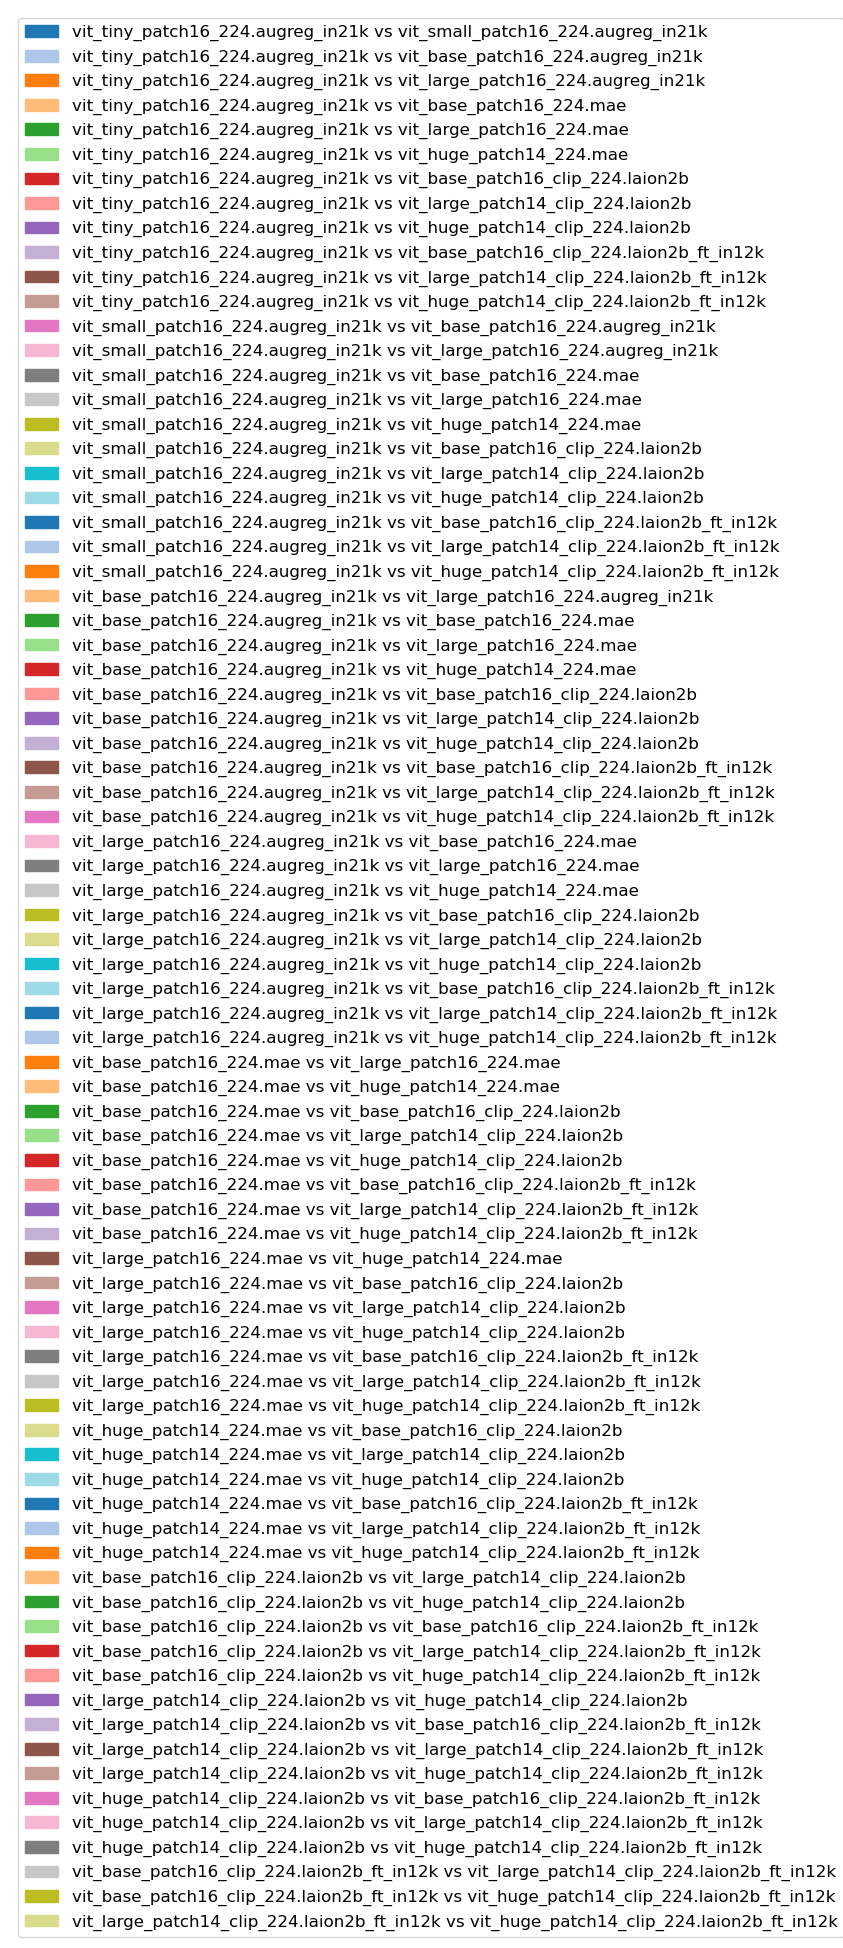
\includegraphics[width=0.7\textwidth]{legend_models.png}
    \caption{Legend showing the names of individual ViT models used in the study. Each model is uniquely represented to facilitate distinction in the alignment plots, providing a reference for identifying alignment patterns.}
    \label{fig:legend_models}
\end{figure}

\subsection{Alignment Dynamics During LLM Training}
\begin{figure}[H]
    \centering
    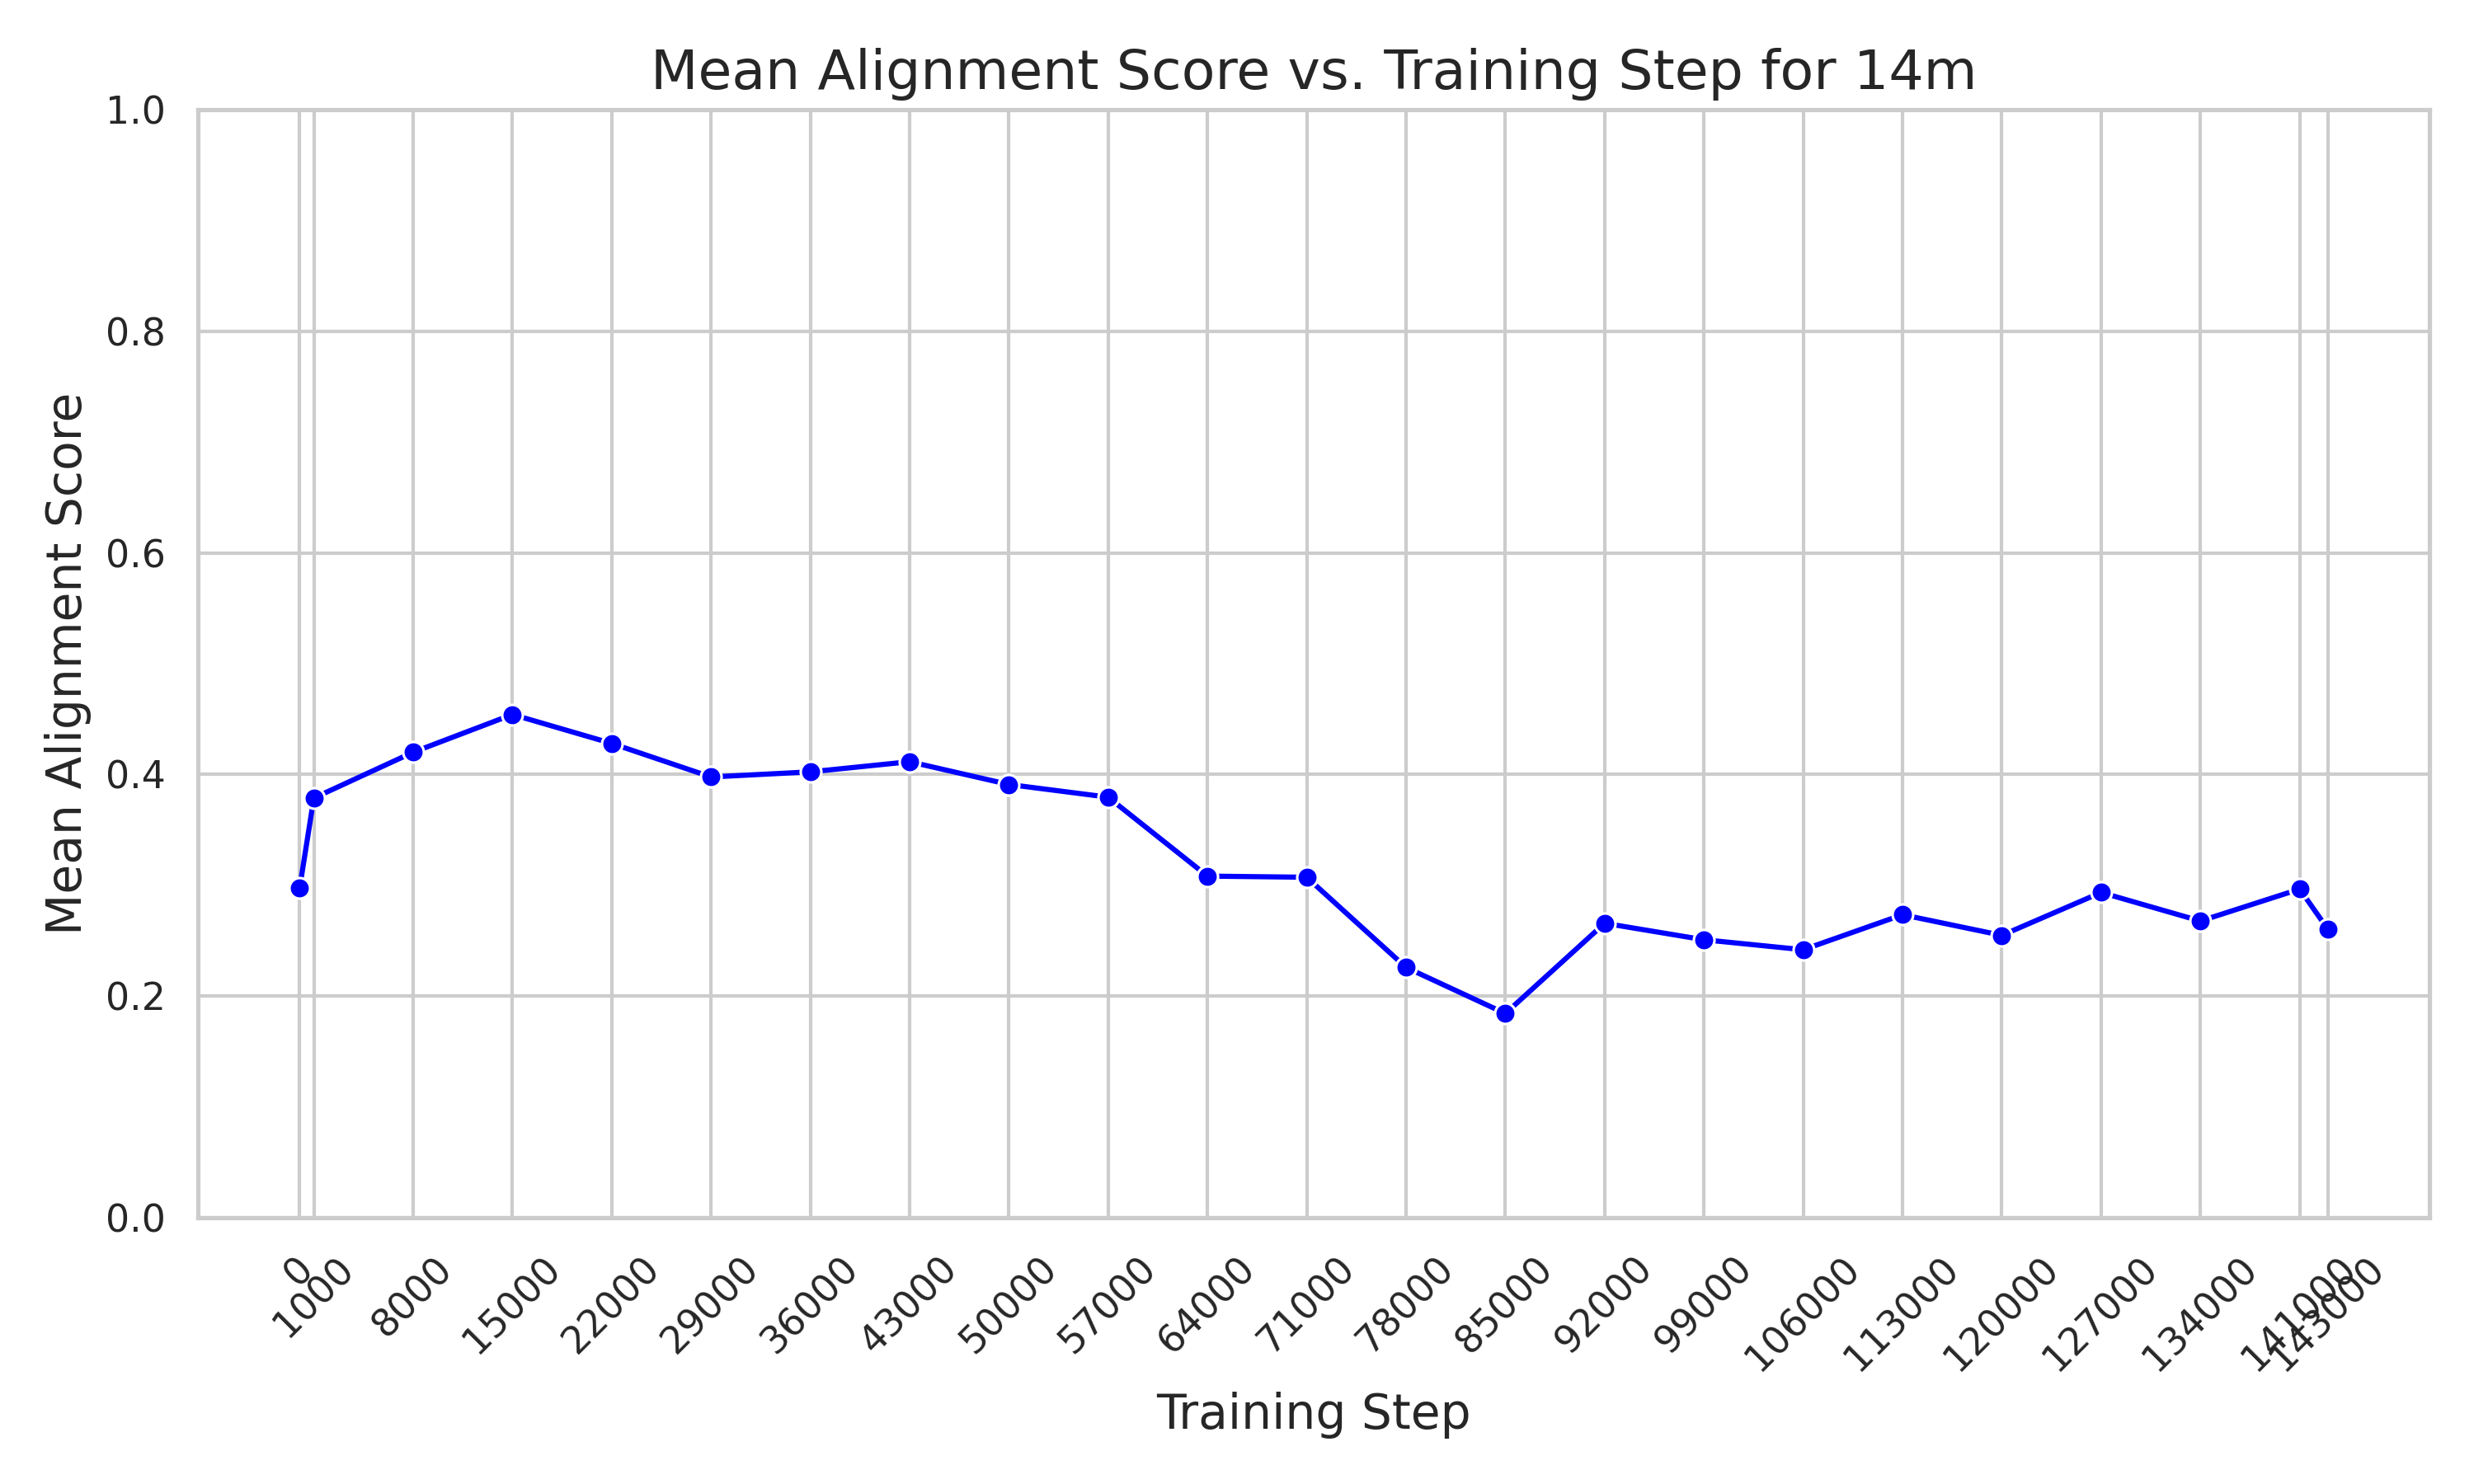
\includegraphics[width=0.48\textwidth]{mean_alignment_score_14m.png}
    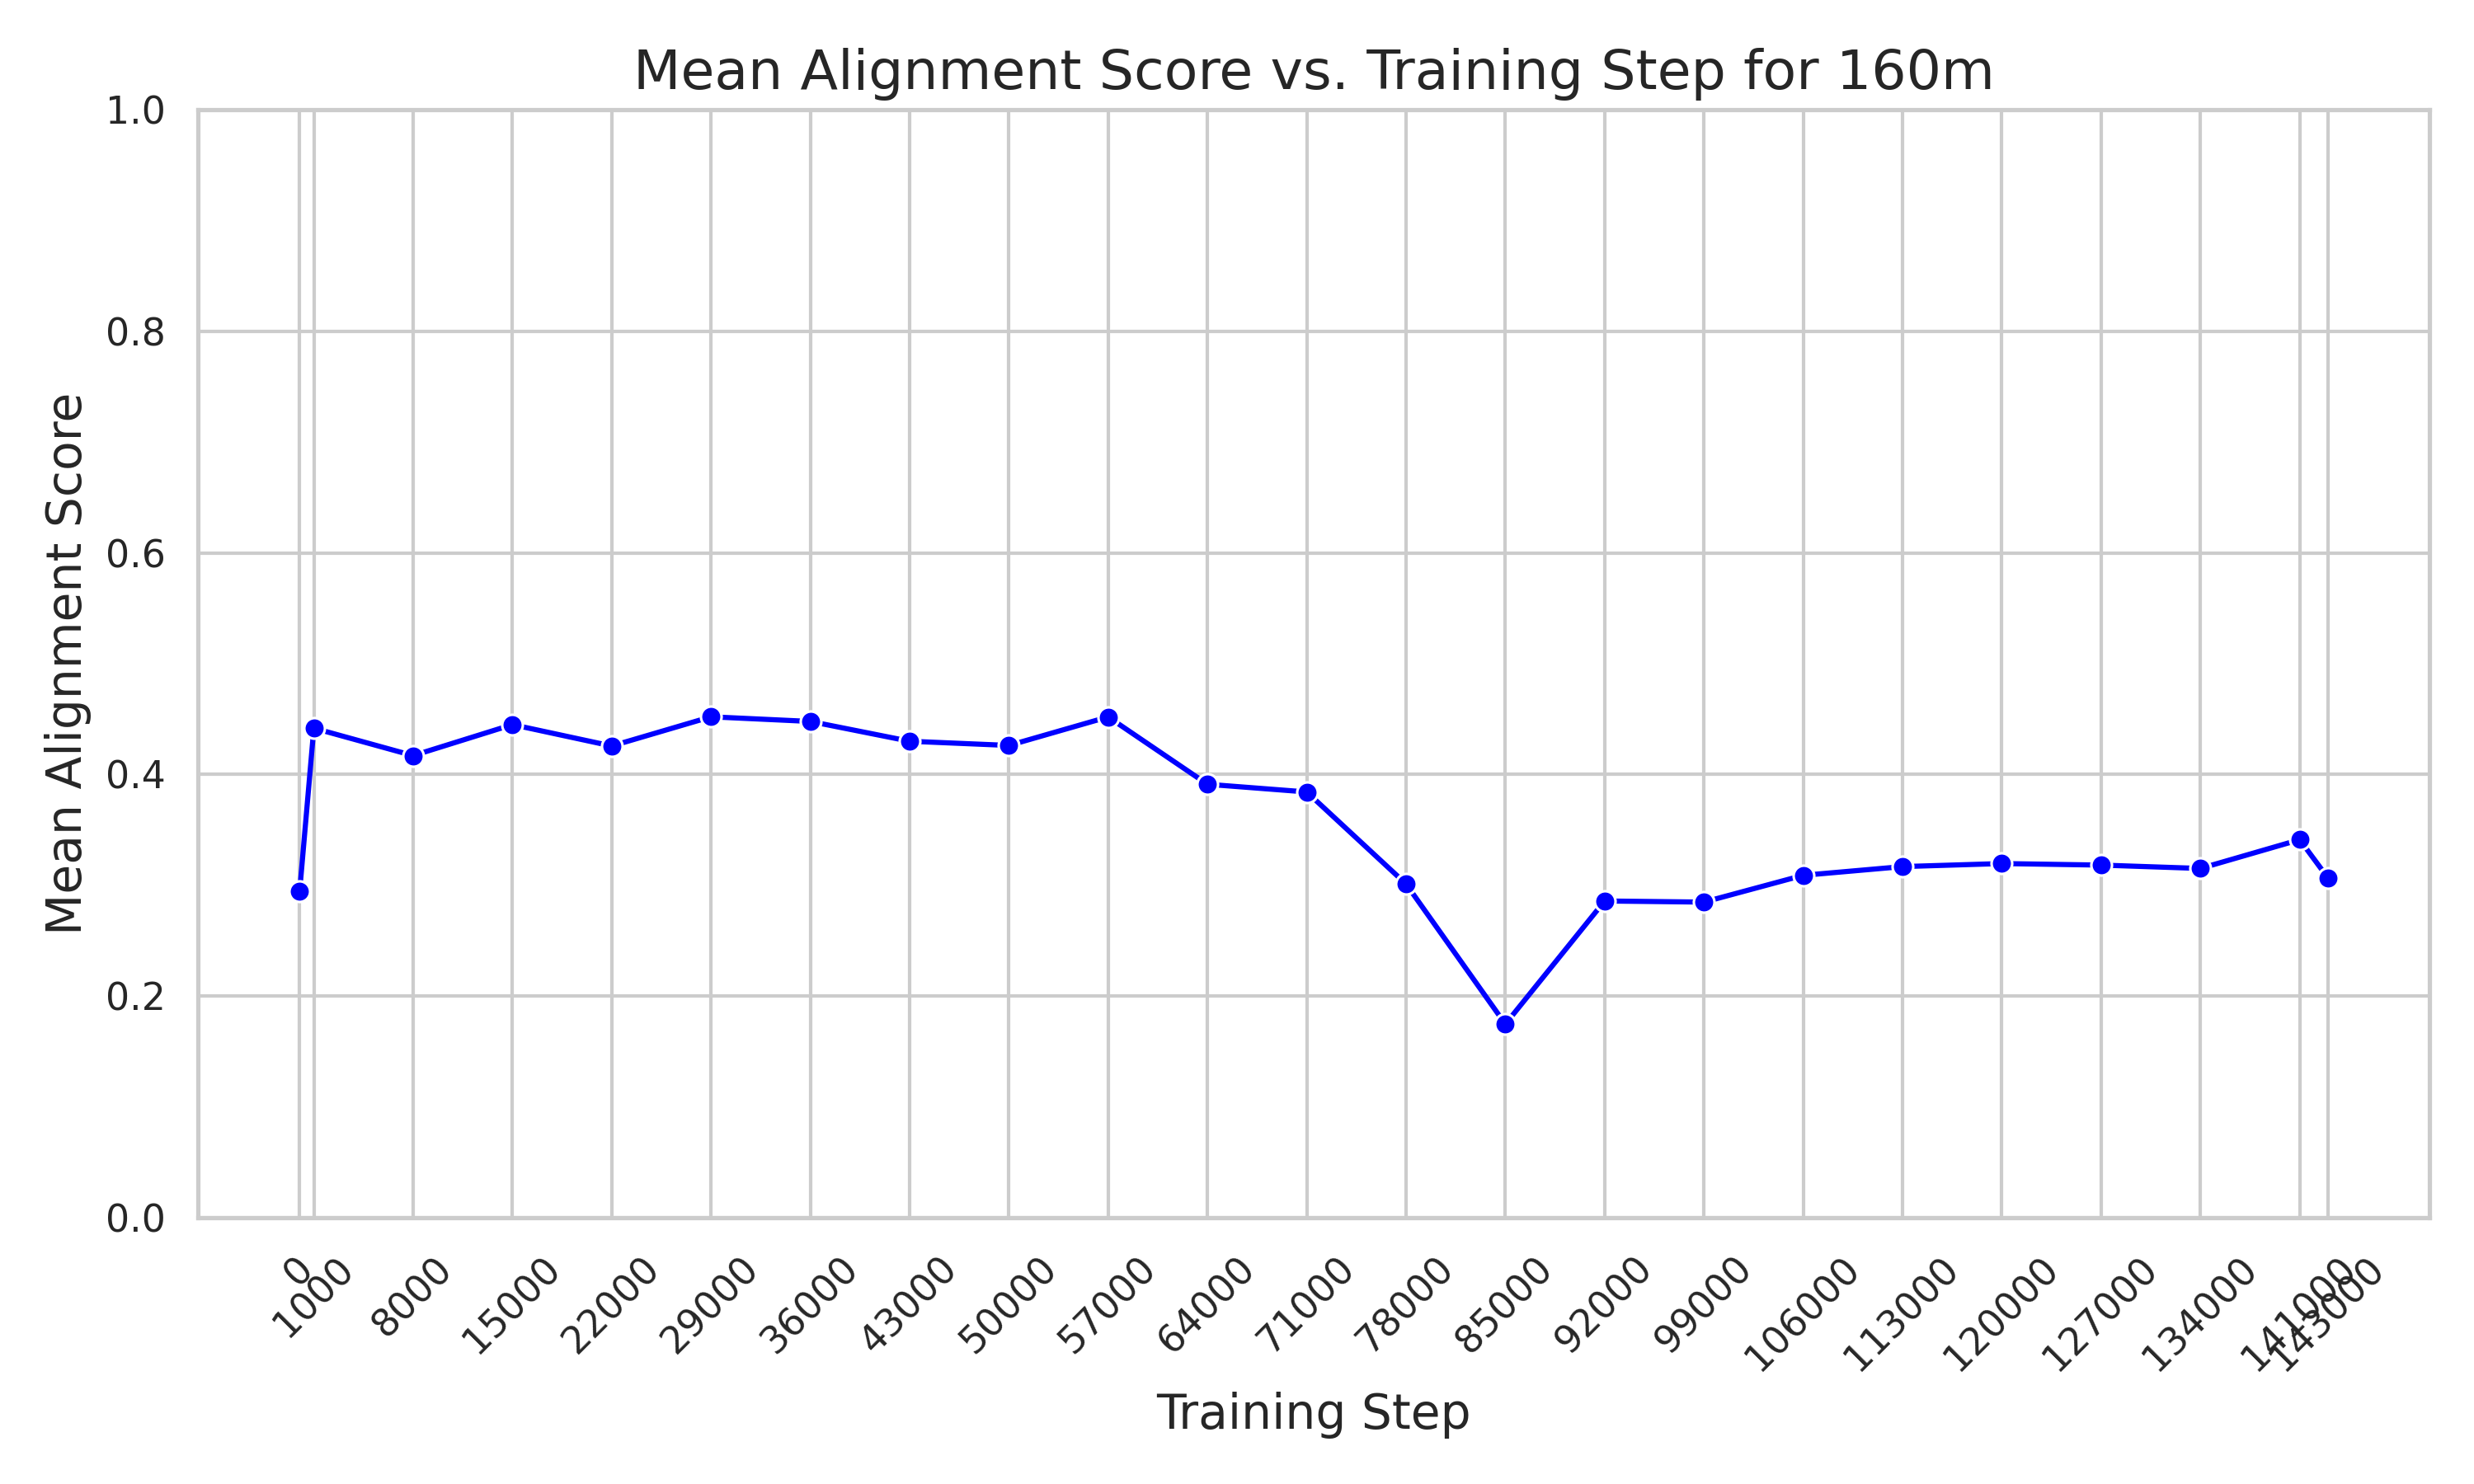
\includegraphics[width=0.48\textwidth]{mean_alignment_score_160m.png}
    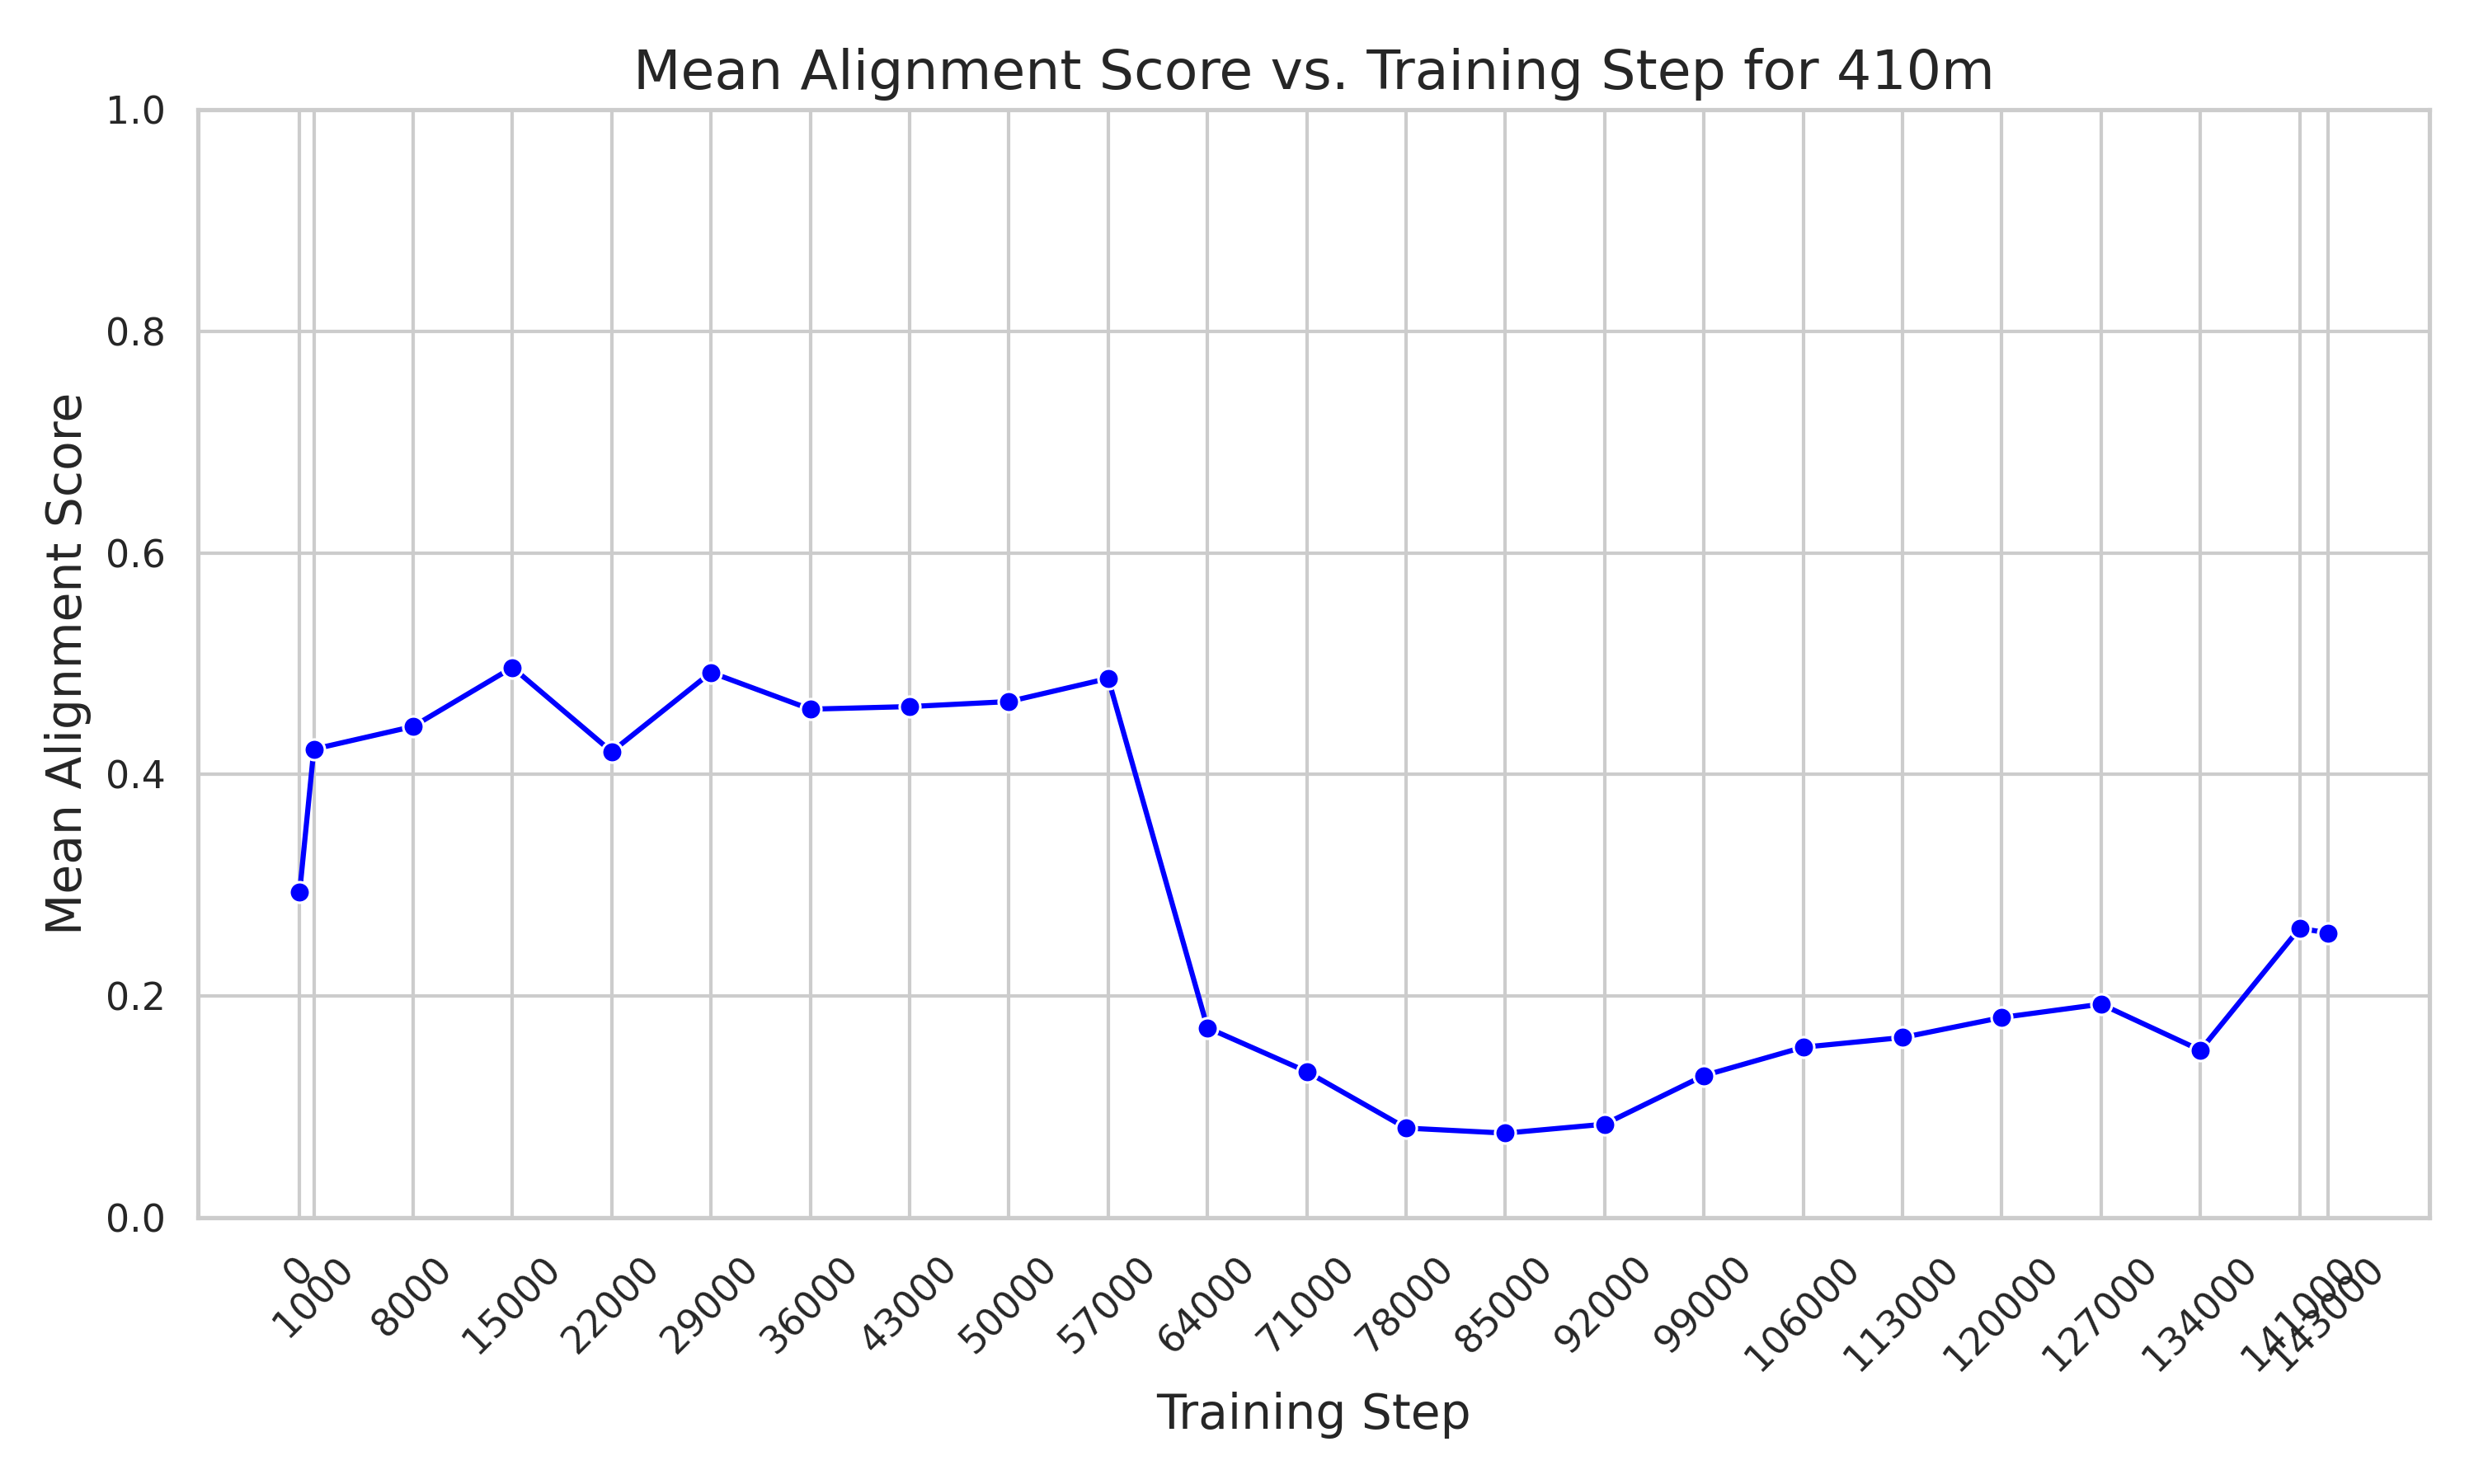
\includegraphics[width=0.48\textwidth]{mean_alignment_score_410m.png}
    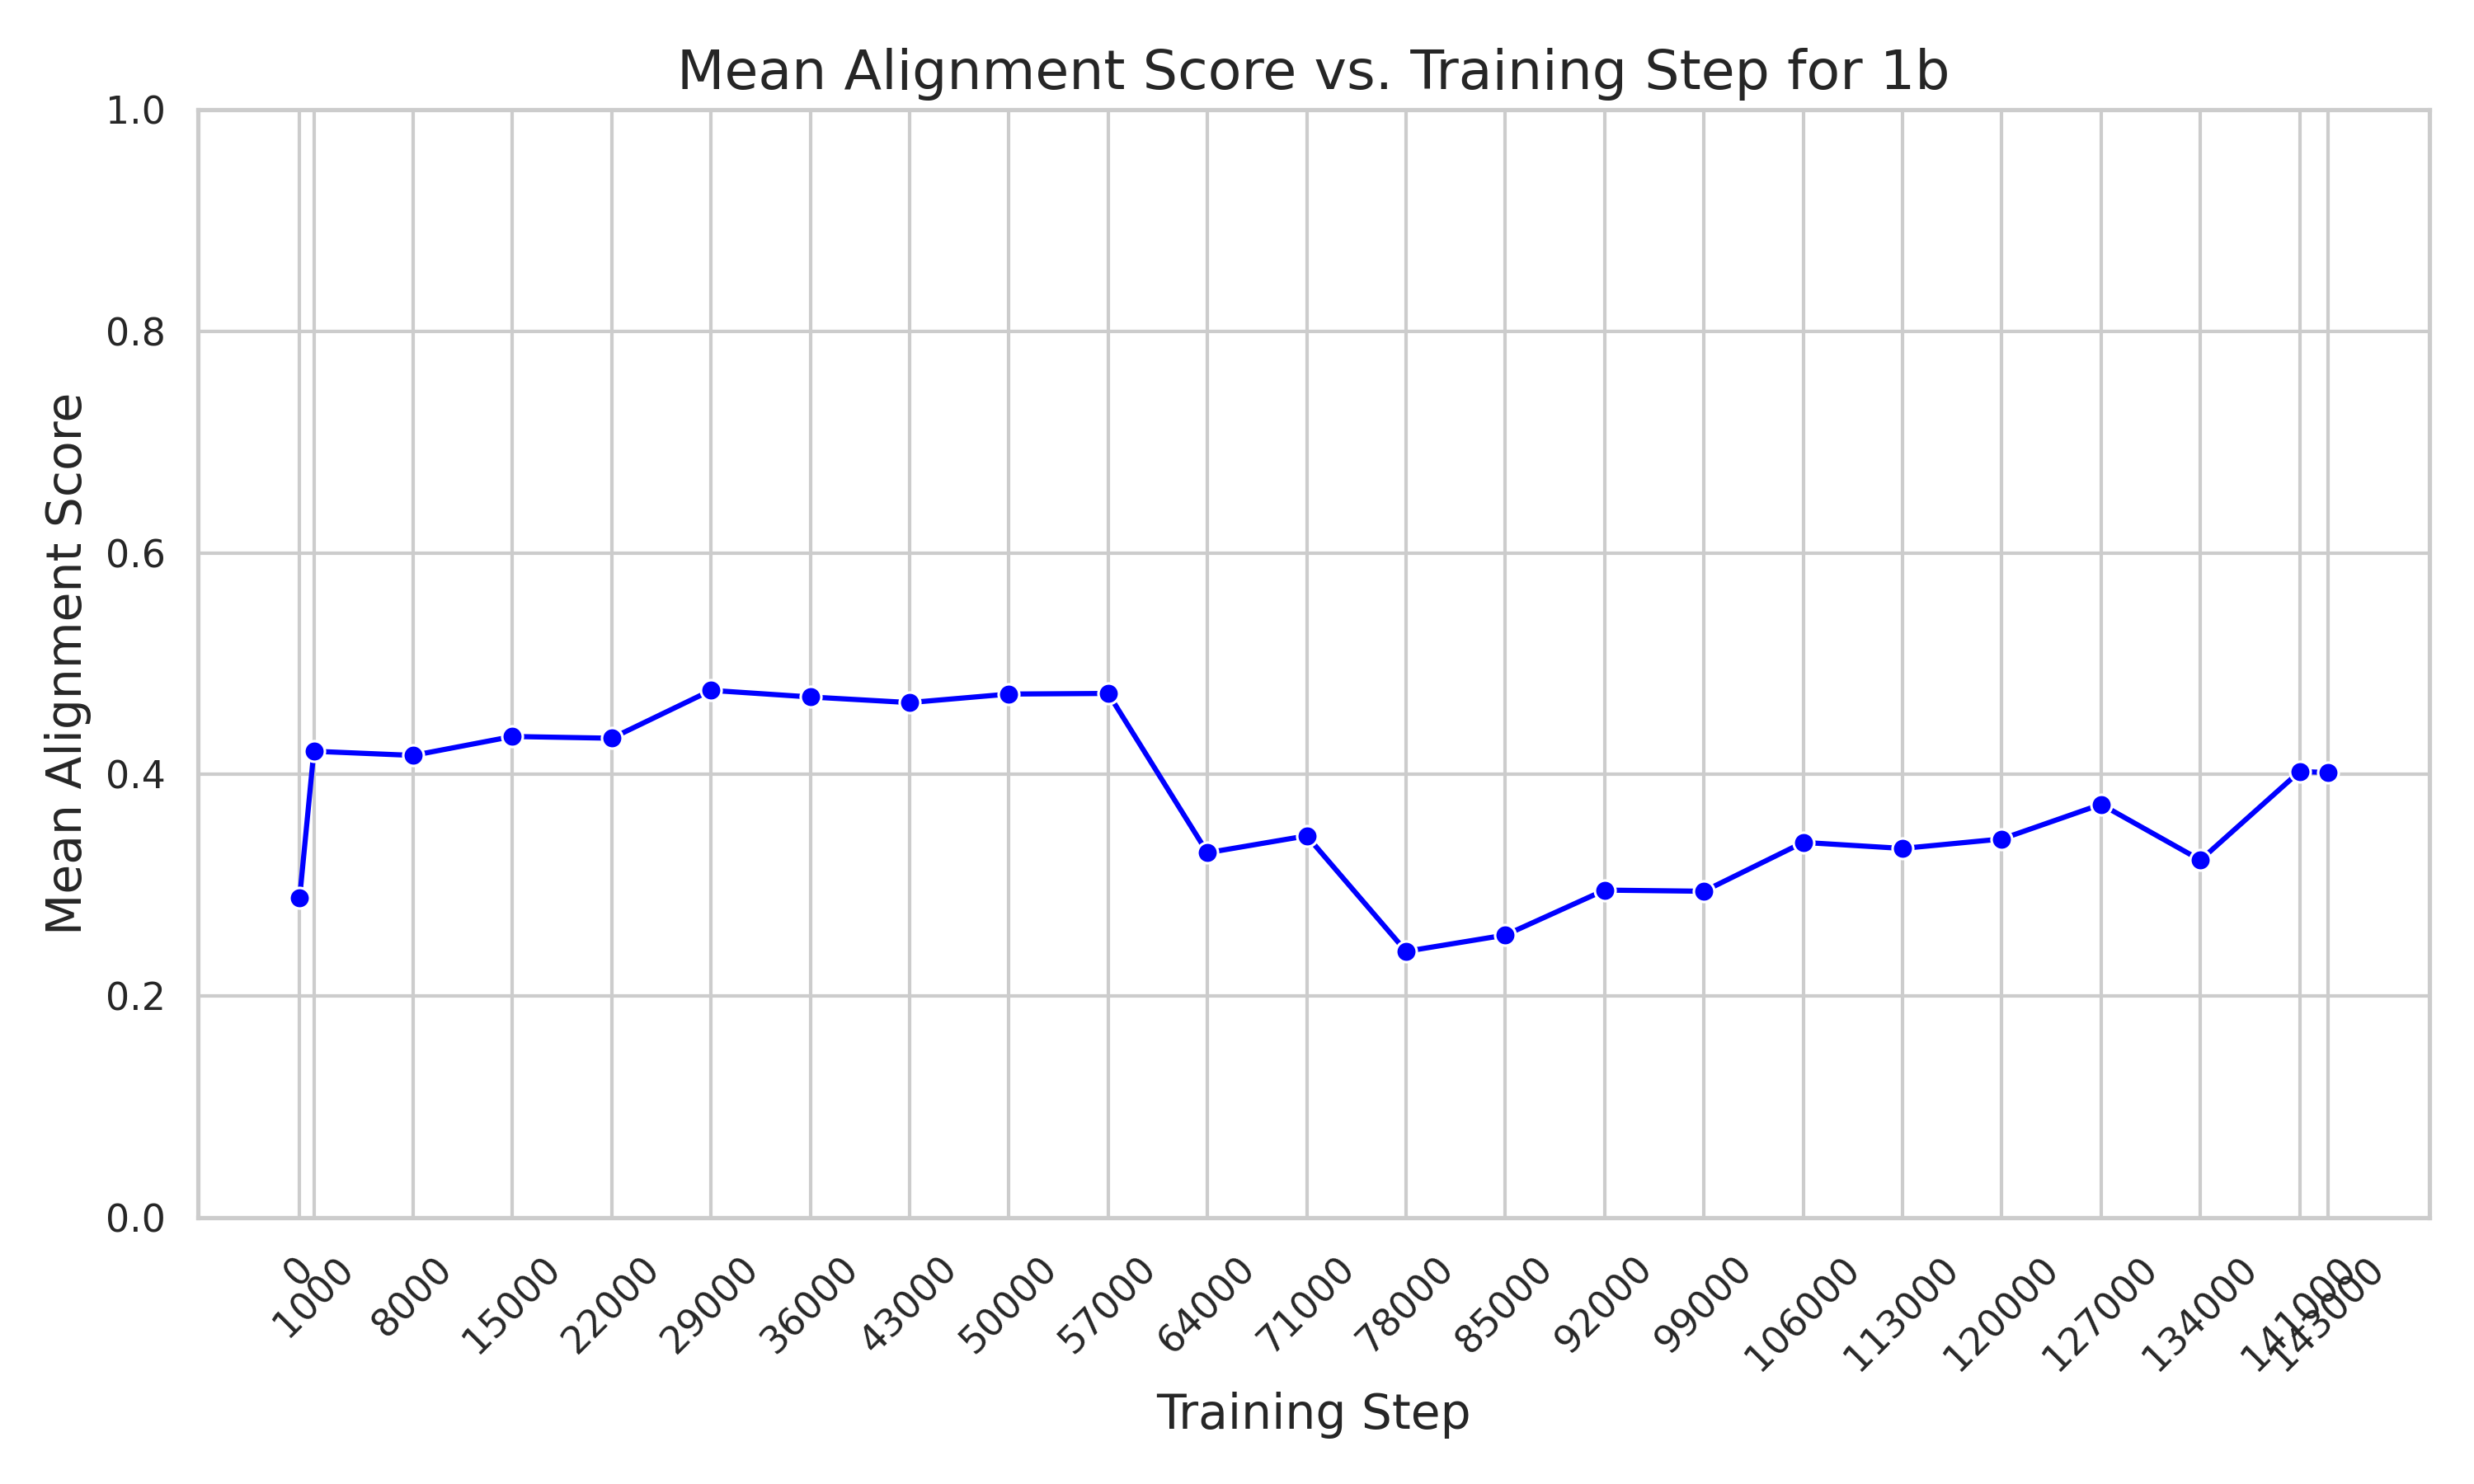
\includegraphics[width=0.48\textwidth]{mean_alignment_score_1b.png}
    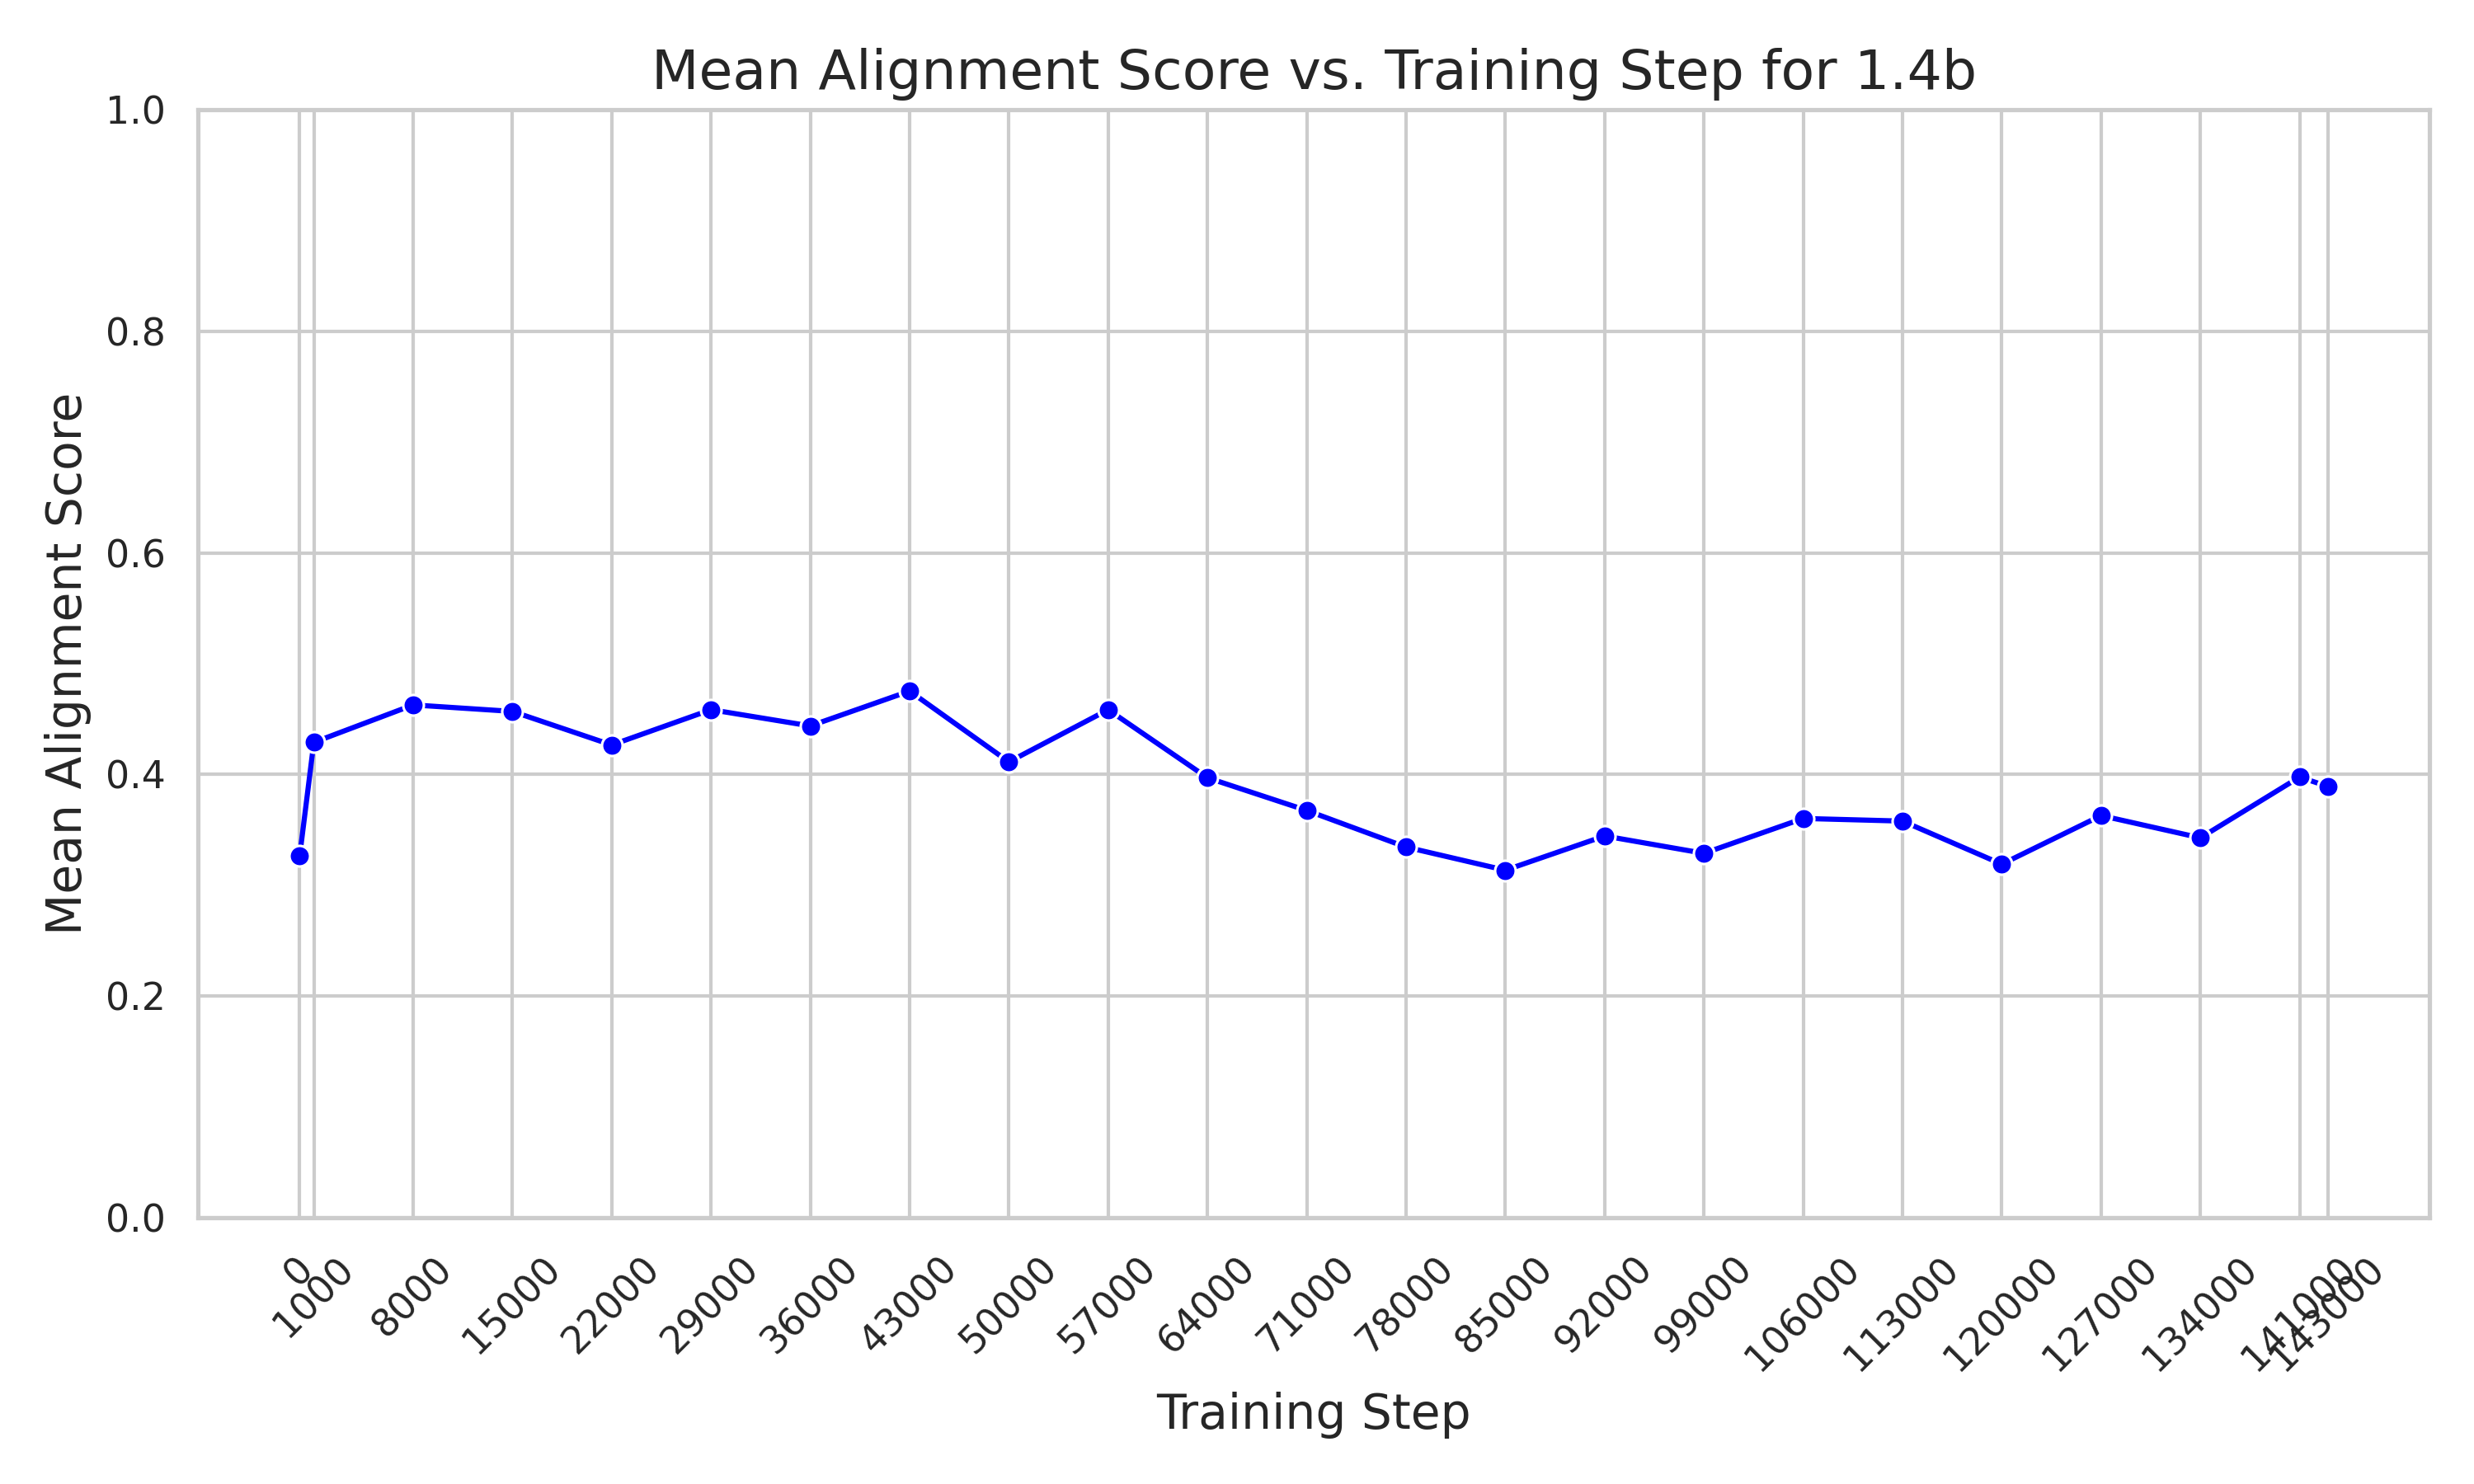
\includegraphics[width=0.48\textwidth]{mean_alignment_score_1.4b.png}
    \caption{Alignment trends of LLMs during training. Scores show non-linear trends across different parameter sizes, with initial similarity between smaller and larger models due to similar initialization methods, followed by divergence as larger models form more detailed representations.}
    \label{fig:llm_training_alignment}
\end{figure}

\section{Discussion}
Our results extend understanding of PRH by showing that neural networks maintain representational alignment in OOD contexts but struggle with random data, indicating that shared statistical models depend on structured input. Noise resilience in our experiments highlights models' robustness in interpreting degraded input, though random noise shows the limits of shared representations. Both signal quality and model pretraining show smooth transitions in representational alignment, suggesting a gradual, rather than abrupt, convergence.

\section{Conclusion}
Our study supports the validity of the Platonic Representation Hypothesis in structured, diverse data environments. Findings highlight the importance of data structure in alignment, suggesting further exploration of PRH in multimodal settings and the effects of training strategies on representational convergence.

\vfill
The code for experiments and analysis in this paper is available on GitHub \href{https://github.com/rokosbasilisk/prh-experiments}{here}.

\clearpage
\begin{thebibliography}{9}

\bibitem{huh2024prh}
Huh, M., Cheung, B., Wang, T., \& Isola, P. (2024). The Platonic Representation Hypothesis. \emph{International Conference on Machine Learning}.

\bibitem{hendrycks2021nae}
Hendrycks, D., Zhao, K., Basart, S., Steinhardt, J., \& Song, D. (2021). Natural Adversarial Examples. \emph{CVPR}. \href{https://arxiv.org/abs/2405.07987}{arXiv:2405.07987}.

\end{thebibliography}

\end{document}

